\section*{Appendix}
\label{sec:appendix}

\subsubsection*{Catch the Ball (CTB)}
The Catch the Ball (CTB) game consists of two objects, a ball and a catcher. In each turn the ball's and catcher's horizontal position are randomly initialized. Then, the ball is straight falling down from its starting position and the player has to adapt the catcher's horizontal position (via 3 inputs: move left/right or stay) so that the ball is "captured" (i.e. $x_{ball} = x_{catcher}$). The visual representation of the CTB game is shown in \ref{fig:catch_the_ball}. 

\begin{Figure}
\begin{center}
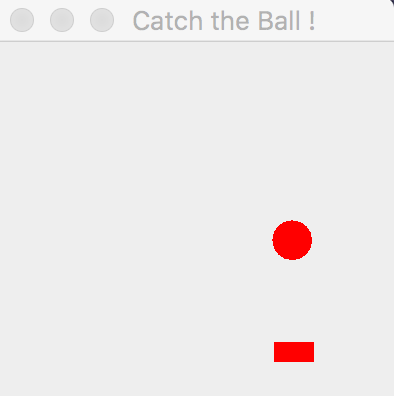
\includegraphics[width=4cm]{imgs/catch_the_ball.png}
\end{center}
\captionof{figure}{Test game - Catch the Ball.}
\label{fig:catch_the_ball}
\end{Figure}

In CTB the possible states are defined by the discrete distance between catcher and ball, which results in $2 width_{board}$ states. Combined with three actions (moving left, right or staying) we have 600 possible state-action-pairs, assuming a game board with of 200. Here, after roughly 10000 training games a well defined Q(s,a) matrix is obtained resulting in a well-performing agent.

\subsection*{Further Diagrams}


\begin{Figure}
\begin{center}
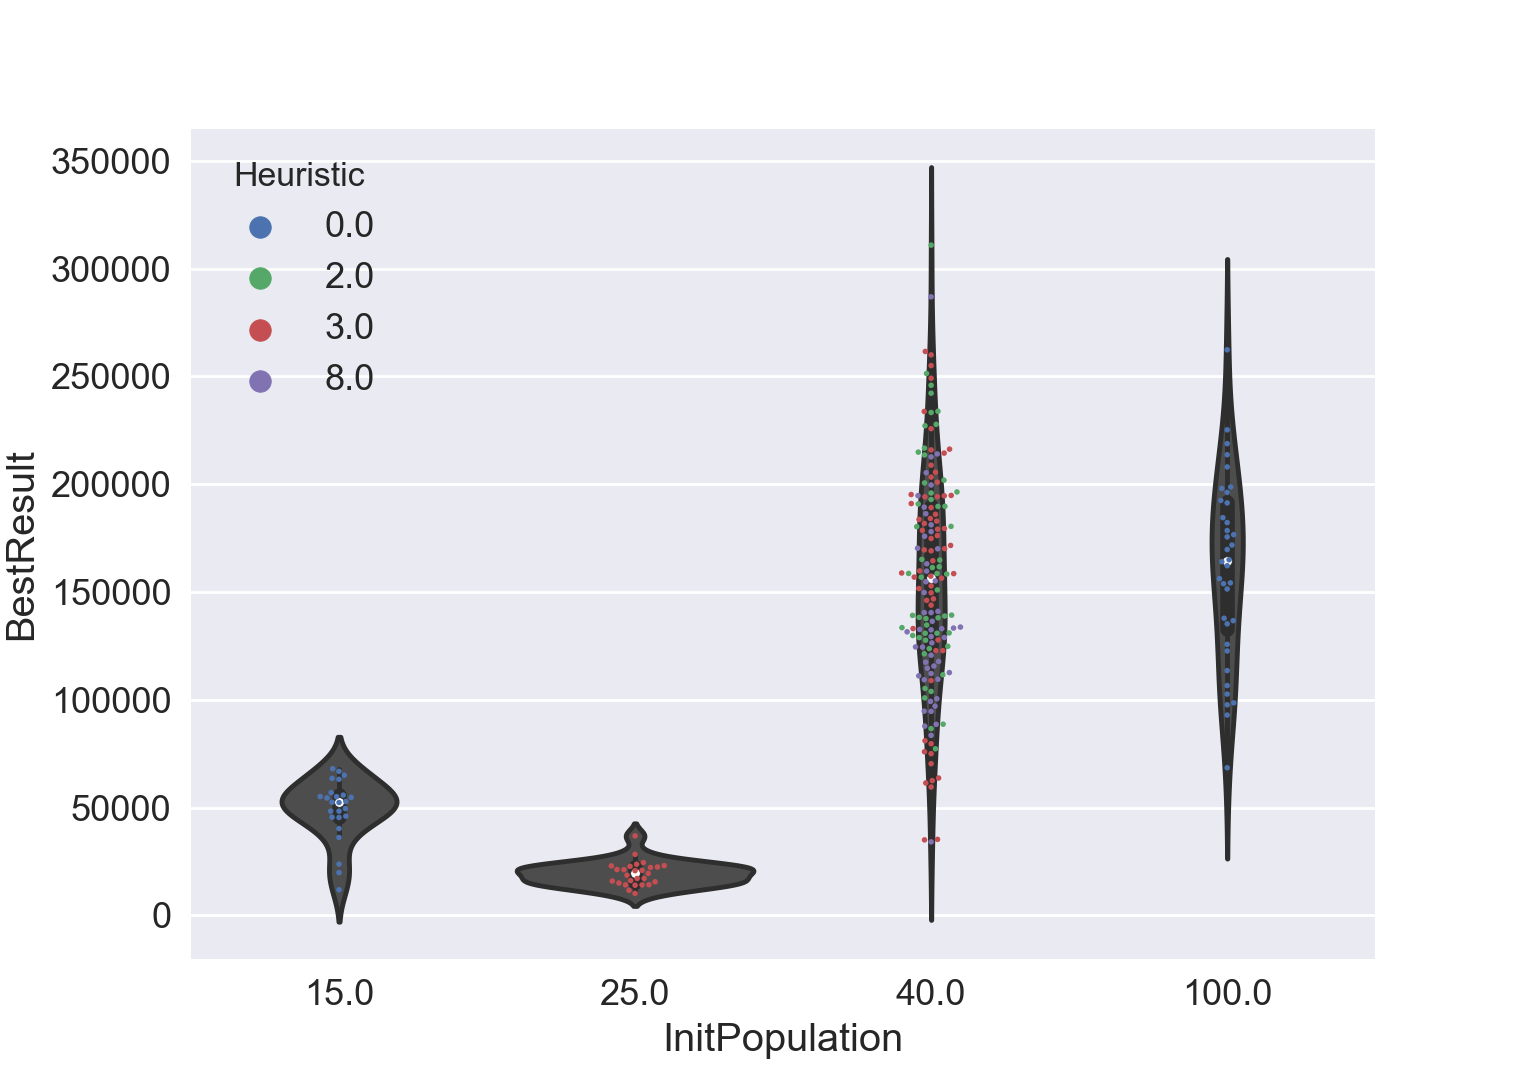
\includegraphics[width=7cm]{imgs/InitPop_Best.png}
\end{center}
\captionof{figure}{Comparison of initial population.}
\label{fig:initpop_best}
\end{Figure}